\section{Spin-2: shape splitting and continuous bifurcation}

\label{sec:5}

\subsection{The quintet and its axial splitting}

Write $h=q_AT_A$, where $T_A$ is the orthonormal symmetric traceless basis of Appendix C. At $\omega=0$ the scalar controls multiply the shape action by $\mathcal K$ and add a shape-independent constant. At the round point its Hessian is $8\mathcal K\delta_{AB}$, so all five normalized directions have the same positive curvature. For the axial reference $M_0=\mathrm{diag}(a,a,a^{-2})$, with $a=(1+\epsilon)^{1/3}$, $\epsilon>-1$, use the paths $M=M_0e^{q_AT_A}$ one at a time. Their curvatures split into a singlet and two doublets:

\begin{equation}\tag{T1}\label{eq:T1}
\begin{aligned}
H_0&=\frac{8\mathcal K(4-a^6)}{3a^8},\\
H_2&=\frac{8\mathcal K(2a^6-1)}{a^2},\qquad (T_2,T_3),\\
H_1&=\frac{4\mathcal K(a^6+1)}{a^8},\qquad (T_4,T_5).
\end{aligned}
\end{equation}

At $a=1$ these agree with the round value. Residual rotations in the 01 plane rotate $(T_2,T_3)$ with twice the angle and $(T_4,T_5)$ with the angle itself. The specified exponential path fixes the meaning of the second derivatives. Off a stationary shape, another path with the same tangent can have a different second derivative, as derived in Appendix D. In particular, the zero of $H_0$ at $\epsilon=1$ is a curvature zero along that path.

\begin{figure}[htbp]
\centering
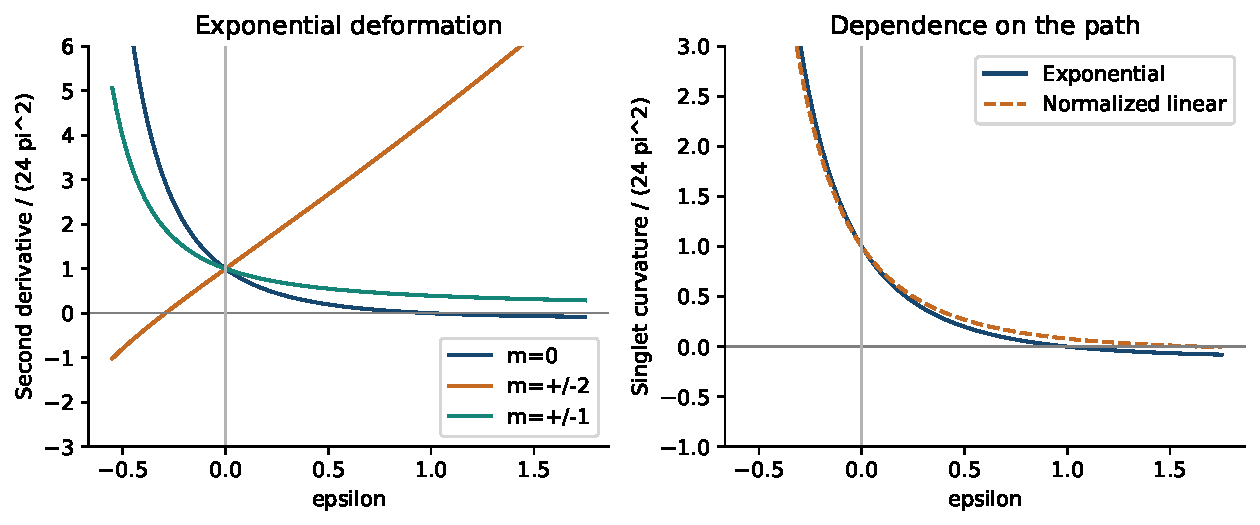
\includegraphics[width=0.93\linewidth]{figures/v3/fig05_shear.pdf}
\caption{The singlet and two doublet curvatures, normalized by $24\pi^2$ at $r=3$, $L=\kappa=1$. The second panel compares two paths with the same tangent at the axial background.}\label{fig:fig05_shear}
\end{figure}

\subsection{Exact doublet minimization at fixed axial control}

Fix $a$ and minimize over the full doublet, $M=M_0\exp(q_2T_2+q_3T_3)$. Let $\rho=(q_2^2+q_3^2)^{1/2}$. The eigenvalues of $S$ are $a^2e^{\sqrt2\rho},a^2e^{-\sqrt2\rho},a^{-4}$. Thus $z=2\cosh(\sqrt2\rho)\ge2$ reduces the problem to a convex quadratic:

\begin{equation}\tag{T2}\label{eq:T2}
F(a,z)=a^4(z^2-4)-2a^{-2}z+a^{-8}
=a^4(z-a^{-6})^2-4a^4.
\end{equation}

\begin{equation}\tag{T3}\label{eq:T3}
\begin{aligned}
\rho_{\ast}(a)&=
\begin{cases}
0,&a^6\ge1/2,\\
\mathrm{arcosh}(1/(2a^6))/\sqrt2,&a^6<1/2,
\end{cases}\\
F_{\min}(a)&=
\begin{cases}
a^{-8}-4a^{-2},&a^6\ge1/2,\\
-4a^4,&a^6<1/2.
\end{cases}
\end{aligned}
\end{equation}

The critical control is $\epsilon_c=1/\sqrt2-1$. For $\epsilon<\epsilon_c$ the minimum has three unequal shape eigenvalues; it approaches the axial shape continuously at the boundary. More precisely,

\begin{equation}\tag{T4}\label{eq:T4}
\begin{aligned}
\rho_{\ast}&=2^{3/4}\sqrt{\epsilon_c-\epsilon}
+O((\epsilon_c-\epsilon)^{3/2}),\\
[\,\partial_\epsilon^2 F_{\min}\,]_{\mathrm{right}}
-[\,\partial_\epsilon^2 F_{\min}\,]_{\mathrm{left}}
&=32\,2^{1/3}.
\end{aligned}
\end{equation}

Both $F_{\min}$ and its first derivative are continuous at $\epsilon_c$. The quartic coefficient in the local expansion in $\rho$ is $2\,2^{1/3}>0$ at criticality. These facts characterize a continuous bifurcation of constrained shape minima, or a continuous shape transition within this finite-dimensional minimization problem.

\begin{figure}[htbp]
\centering
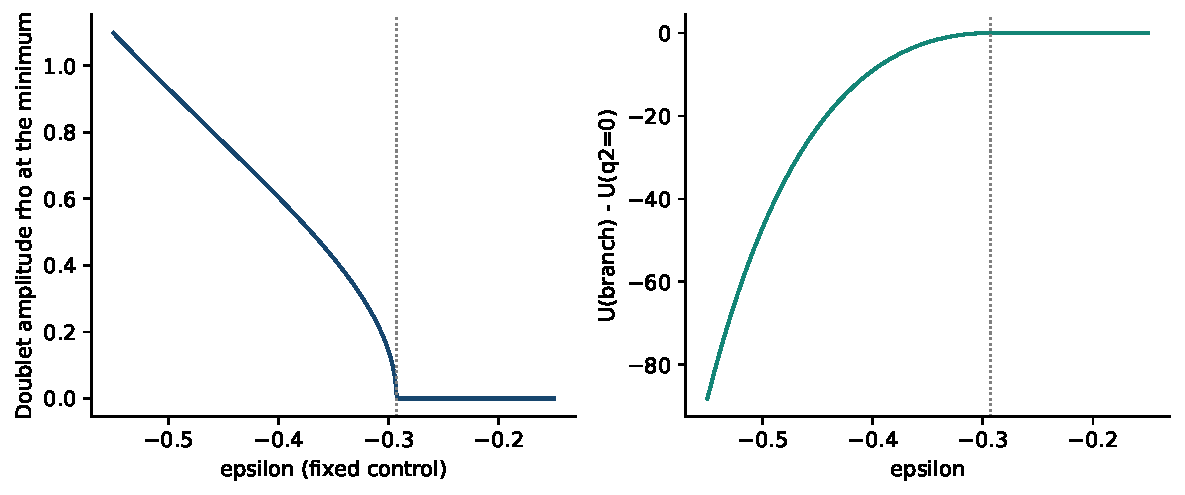
\includegraphics[width=0.93\linewidth]{figures/v3/fig06_branch.pdf}
\caption{Doublet amplitude and the potential gain at fixed axial control. The dotted line is $\epsilon_c$. For nonzero amplitude the minimizers form a rotation orbit, not two isolated minima.}\label{fig:fig06_branch}
\end{figure}

The two signs of $q_2$ on the cut $q_3=0$ are points on the circle $q_2^2+q_3^2=\rho_{\ast}^2$. Residual $SO(2)$ rotations connect that circle. When shapes related by rotations and axis relabeling are identified, it represents one triaxial shape class at each fixed control.

\subsection{Global minimum of the static shape potential}

At fixed scalar controls and zero twist, every positive-definite $S$ of determinant one has an eigenvalue representation of the form used in (T2), after choosing an axis order. Minimizing (T3) also over $a>0$ therefore covers all shapes, modulo rotations. For $a^6<1/2$, $F_{\min}>-2^{4/3}>-3$. On the complementary branch,

\begin{equation}\tag{T5}\label{eq:T5}
F_{\min}+3=
\frac{(a^2-1)^2(3a^4+2a^2+1)}{a^8}\ge0.
\end{equation}

Equality requires $a=1,z=2$, hence $S=I$. On this zero-twist slice, the round shape is the unique global minimizing shape of the static potential, modulo rotations. Since the twist term in (M3) is nonnegative, minimizing over twist as well gives $\omega=0$. At a prescribed nonzero twist, the shape dependence of the last term in (M3) generally shifts the shape minimum. The fixed-control bifurcation and the full-shape minimum above are complementary results of the static zero-twist potential. At fixed torsion and circle circumference, combining this bound with Section 3 also selects the round radius minimum when $V\ne0$ and $\eta^2<4$.

\begin{figure}[htbp]
\centering
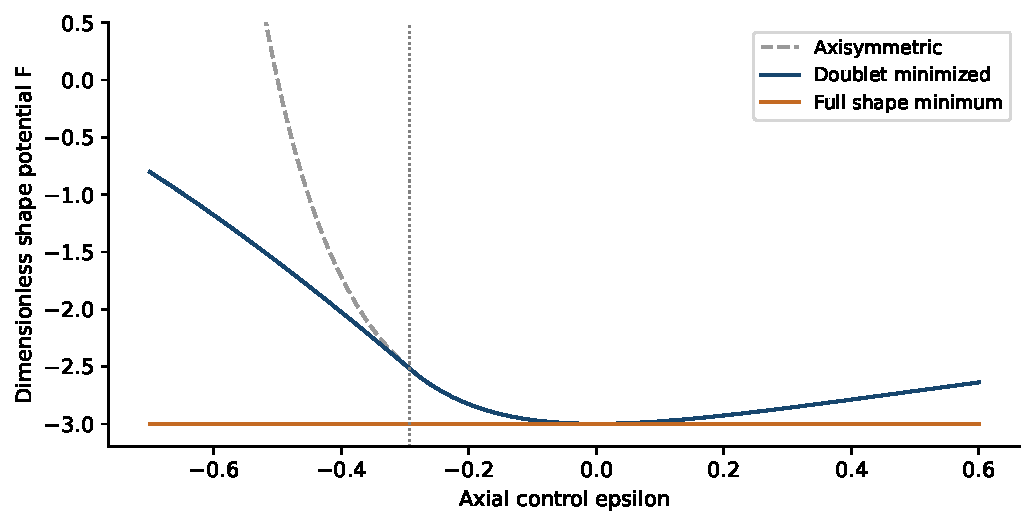
\includegraphics[width=0.93\linewidth]{figures/v3/fig07_shape_minima.pdf}
\caption{The axial shape potential, its doublet-minimized value and the full-shape lower bound $F=-3$. Releasing the axial control selects $\epsilon=0$, $\rho=0$.}\label{fig:fig07_shape_minima}
\end{figure}

\subsection{Circle-dependent shape}

Set $\omega=0$ and write $B=M^{\mathsf T}M$, with $\det B=1$. Then $Y=0$ and $\mathrm{tr}(B^{-1}B')=0$. The derivative part of (M6) becomes

\begin{equation}\tag{T6}\label{eq:T6}
\mathcal L_{\partial}\big|_{\omega=0}
=-\frac{3\pi^2r(r')^2}{4\kappa^2L}
+\frac{\pi^2r^3}{32\kappa^2L}
\mathrm{tr}\!\left[(B^{-1}B')^2\right].
\end{equation}

The shape term is nonnegative: $B^{-1}B'$ is similar to the symmetric matrix $B^{-1/2}B'B^{-1/2}$. Near a constant round reference, $M=e^h$ gives the quadratic coefficient $\pi^2r_0^3\mathrm{tr}[(h')^2]/(8\kappa^2L_0)$. The scalar--shape derivative cross term vanishes exactly at zero twist. Thus the static bifurcation and a positive shape derivative cost can be described in the same sector. Their extension to nonzero twist requires the joint terms of Section 6.
